\chapter{Introducción a los diagramas de secuencia}
\label{ch:msc}

En este capítulo realizamos una introducción a los diagramas de
secuencia. Explicaremos el lenguaje gráfico utilizado y ofreceremos el
significado informal de algunas de sus construcciones. Termina el
capítulo con una descripción algo más detallada de aquellas
construcciones de los diagramas de secuencia tratados en este trabajo.

\section{Lenguajes de descripción de escenario}
Los lenguajes gráficos de descripción de escenarios se utilizan
ampliamente en el desarrollo de software para representar escenarios
de uso típico del sistema, comportamientos prohibidos en el sistema,
casos de prueba, etc. Existen múltiples variantes de estos lenguajes.
todos ellos siguen una sintaxis gráfica similar y se engloban bajo
nombres como
\begin{itemize}
\item diagramas de secuencias de mensajes (\emph{Message Sequence Charts}),
\item diagramas de secuencia de vida (\emph{Live Sequence Charts}),
\item diagramas de interacción (\emph{Interaction Diagrams}),
\item diagramas de secuencia (\emph{Sequence Diagrams}),
\item diagramas de colaboración (\emph{Collaboration Diagrams}),
\item etc.
\end{itemize}

De algún modo, tantos nombres parecen un reflejo de un problema
evidente. Exageramos: si pedimos a dos ingenieros dibujar el mismo
escenario utilizarán lenguajes parecidos pero diferentes. Si además
esos escenarios son complejos las diferencias se acrecentarán y, lo
peor de todo, puede que no estén de acuerdo en el significado de lo
que escriben.

La figura~\ref{fig:intromsc:discrepancias} muestran algunos ejemplos
de escenarios encontrados en Internet.

http://modeling-languages.com/
http://modeling-languages.com/dibujando-diagramas-de-secuencia-estilo-servilleta/

Scenario languages are widely used in software development. Typical
usage scenarios, forbidden behaviors, test cases and many more aspects
can be depicted with graphical scenarios. Several language variants
were proposed over the years. The International Telecommunication
Union’s (ITU) Message Sequence Chart (MSC) [6] was one of the first of
such languages. It is widely used, since its first introduction in
1993 it was updated several times, and the specification defines also
a formal semantics for the basic elements of the language based on
process theory. Triggered Message Sequence Charts (TMSC) [8] proposed
extensions to MSC to express conditions and refinement in a precise
way. Live Sequence Charts (LSC) [9] concentrated on distinguishing
possible and necessary behaviors. A special technique and a tool, the
Play-Engine, were also developed for LSC to specify reactive systems
[10].

Los diagramas de secuencia, en sus diferentes variantes, se usan
intensivamente para la descripción de sistemas (no solo sistemas
software). Con ellos suelen describirse escenarios de uso típico del
sistema, comportamientos prohibidos en el sistema, casos de prueba,
etc. Podríamos decir que se han convertido en una herramienta
fundamental de comunicación entre los participantes en el desarrollo
de los sistemas (la variante de UML es la segunda notación más usada,
sólo superada por los diagramas de clase
\cite{Dobing:2006:UU:1125944.1125949}).

Antes de continuar, veamos un ejemplo real. El ejemplo es un diagrama
de secuencias escrito utilizando una notación informal, extraído del
capítulo 3 del \emph{subset} 26 de la especificación de requisitos de
sistema de ERTMS/ETCS (\emph{European Raiway Traffic Management System /
  European Train Control System}):
\begin{center}
  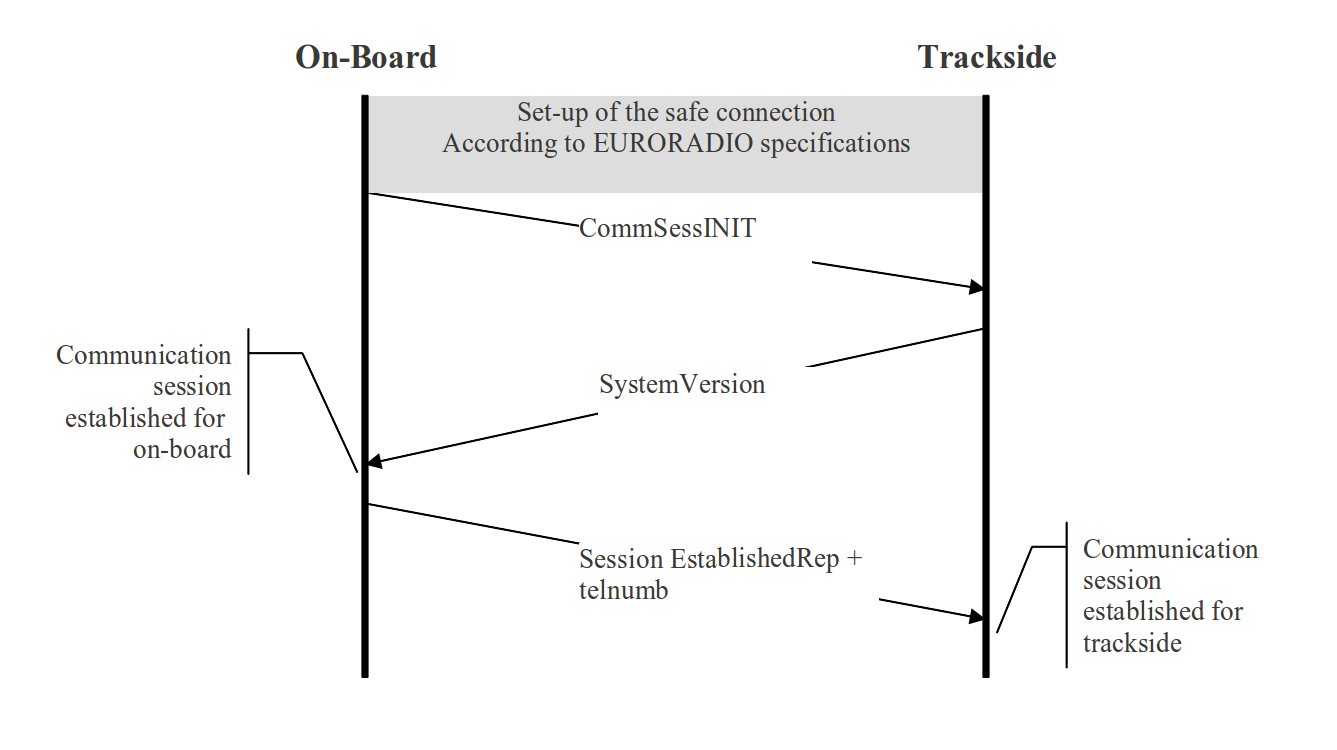
\includegraphics[width=0.9\linewidth]{images/ejemplo-ertms.png}
\end{center}
El diagrama describe un escenario de comunicación entre el sistema
embarcado en el tren y el sistema en la vía que lleva a establecer una
conexión estable entre ambos. Se puede observar que 

\url{http://www.xmlblaster.org/replication/ch02s04.html}
Database Replication
Guide on how to perform Database replication with XmlBlaster
insertSequence.png

\url{http://docs.oracle.com/cd/E15919_01/wlp.1032/e14235/chap_details.htm}
Fusion Middleware Federated Portals Guide for Oracle WebLogic Portal
Federated Portal Architecture
Web Services for Remote Portlets (WSRP).
WSRP Sequence Diagram
procflow.gif

\url{http://www.agilemodeling.com/artifacts/sequenceDiagram.htm}
What Scott W. Ambler calls System-level sequence diagram.
sequenceDiagramSystemLevel.JPG


\url{http://docs.tinyos.net/tinywiki/index.php/TUnit_Test_Flow}
System Sequence Diagrams to illustrate proper use of TUnit. TUnit is a unit testing framework geared for TinyOS and sensor networks. 
\url{System_sequence_diagram.jpg}



\section{Diagramas de secuencia}

Según Bjorner \cite{bjorner}, los diagramas de secuencia (a partir de
ahora MSCs), \todo{AB: aquí me pones la pregunta ''de qué?''. No
  entiendo a que te refieres.} son una notación gráfica para describir
intercambios de mensajes entre entidades. Los MSCs fueron
estandarizados por primera vez por la \textit{CCITT} (conocida ahora
como la \textit{ITU-T}) en \textit{Recommendation Z.120} en 1992,
donde se especificaron sus componentes.
Se realizaron revisiones en 1996, donde se especificó la
forma en que varios MSCs (llamados \textit{Basic} MSC (BMSC) pueden
ser combinados para formar un documento MSC en el cual la relación entre
dichos BMSCs se describe mediante un \textit{high-level} MSC (HMSC), y
en 1999 donde se ofrecen facilidades adicionales para la
especificación de los datos que se pasan dentro de los mensajes, y se
permiten expresiones en línea.

A continuación vamos a hacer un breve resumen sobre los BMSC, que son
los diagramas que vamos a usar en \textit{Progtalk}.

\section{Basic MSCs (BMSCs)}
Un \textit{basic} MSC (a partir de ahora BMSC), esta formado por un
conjunto de instancias. Una instancia~\ref{fig:instances} es una
entidad abstracta en la cual suceden eventos. Una instancia se nota
con un cuadrado vacío, el cual tiene una linea recta que sale
verticalmente y hacia abajo desde su base. Esta recta representa una
linea temporal donde los eventos van ocurriendo por orden cronológico
de arriba hacia abajo. Los eventos que pueden suceder entre instancias son:

\begin{figure}
  \centering
\begin{postscript}
\begin{msc}{Instances}

\declinst{a}{User}{}
\declinst{f}{Agent}{``DHL''}
\declinst{u}{Computer}{}

\end{msc}
\end{postscript}
  \caption{Ejemplo de instancias.}
  \label{fig:instances}
\end{figure}

\subsection*{Acciones}
Son eventos locales a una instancia. Se representan por una caja en la
línea temporal con una etiqueta en su interior. Las acciones se usan
para especificar cambios en el estado interno de la instancia,
\subsection*{Mensajes salientes} 
Representan el envío de un mensaje desde una instancia origen a otra
instancia destino.
\subsection*{Mensajes entrantes}
Representan la recepción de un mensaje. Lógicamente a cada evento de
mensaje saliente le corresponde otro evento de mensaje entrante. A
esto se le conoce como \textit{intercambio de mensajes} y se representa con una
flecha que sale de la línea temporal de la instancia origen a la
línea temporal de la instancia destino. Todo intercambio de mensajes
debe de estar etiquetado con un identificador. Podemos ver un ejemplo
de intercambio de mensajes en la figura~\ref{fig:message_exchange}

\begin{figure}
  \centering
  \begin{postscript}
\begin{msc}{Message exchange}

\declinst{a}{User}{}
\declinst{f}{Agent}{``DHL''}

\mess{``hello''}{a}{f}[3]
\mscmark{t=0}{a}
\nextlevel[3]
\mscmark[br]{t=1}{f}
\nextlevel[3]

\mess{``test1''}{f}{a}[3]
\mscmark{t=4}{f}
\nextlevel[3]
\mscmark[br]{t=10}{a}
\nextlevel[3]

\end{msc}
  \end{postscript}
  \caption{Ejemplo de un intercambio de mensajes en un msc.}
  \label{fig:message_exchange}
\end{figure}

\subsection*{Condiciones}
Describen un estado el cual es común a un conjunto de instancias
dentro del MSC. Su fin es meramente informativo y se representan
mediante hexágonos los cuales se extienden a lo largo de las líneas de
tiempo de las instancias sobre las que la condición se aplica. El
texto de la condición debe ir en el interior del hexágono. Podemos ver
un ejemplo en la figura~\ref{fig:condition}

\begin{figure}
  \centering

  \begin{postscript}
\begin{msc}{Conditions}

\declinst{u}{User1}{``Client''}
\declinst{f}{User2}{``Server''}

\condition{some condition}{u,f}
\nextlevel[3]
\mess{``hello''}{u}{f}
\nextlevel
\action{a}{f}
\nextlevel
\condition{C}{u}
\nextlevel[2]
\condition{A,B,C}{u,f}
\nextlevel[2]

\end{msc}
\end{postscript}

  \caption{Ejemplo de una condicion dentro en un msc.}
  \label{fig:condition}
\end{figure}

\subsection*{Temporizadores}
Estos eventos son locales a las instancias y como su propio nombre
indica sirven para controlar la ocurrencia temporal de los eventos
como vemos en la figura~\ref{fig:timer}. Se
nota con un reloj de arena.

\begin{figure}
  \centering
\begin{postscript}
\begin{msc}{Timers}

\declinst{u}{User1}{``Client''}
\declinst{f}{User2}{``Server''}

\settimer{T,50}{f}
\nextlevel[2]
\mess{``hello''}{f}{u}[1]
\nextlevel[2]
\timeout{T}{u}

\end{msc}
\end{postscript}

  \caption{Ejemplo de un temporizador dentro en un msc.}
  \label{fig:timer}
\end{figure}

\subsection*{Procesos de creación de instancias} 
Evento donde una instancia crea a otra nueva. Podemos ver un ejemplo
en la figura~\ref{fig:instanceprocess}
\begin{figure}
  \centering

  \begin{postscript}
\begin{msc}{Timers}

\declinst{u}{User1}{Client}
\dummyinst{f}{}{}
\declinst{k}{User3}{Admin}

\mess{``request''}{u}{k}
\nextlevel[3]
\create{kick}{k}{f}{}{f}
\nextlevel
\stop{k}
\nextlevel[2]
\mess{``OK''}{f}{u}
\nextlevel
\stop{f}
\nextlevel[2]
\create{start}[b]{u}[.75]{k}{}{again}
\nextlevel[2]

\end{msc}    
  \end{postscript}
  \caption{Ejemplo de procesos de creación y terminación de instancias.}
  \label{fig:instanceprocess}
\end{figure}
\subsection*{Procesos de terminación de instancias}
Evento donde una instancia se termina a si misma. Podemos ver un ejemplo
en la figura~\ref{fig:instanceprocess}
\subsection*{Corregiones}
Son partes de la línea temporal de una instancia donde la premisa de
que los eventos ocurran de forma estrictamente temporal deja de ser
indispensable. Se notan con una línea discontinua y podemos ver un
ejemplo en la figura~\ref{fig:region}.

\begin{figure}
  \centering
  \begin{postscript}
\begin{msc}{Communication}

\declinst{u}{User1}{``Client''}
\declinst{f}{User2}{``Server''}
\declinst{k}{User3}{``Admin''}

\regionstart{activation}{u}
\nextlevel[3]
\regionend{u}
\mess{``hello''}{u}{f}
\nextlevel
\regionstart{coregion}{f}
\nextlevel
\regionstart{suspension}{k}
\mess{``bye''}{f}{k}
\nextlevel
\regionstart{activation}{u}
\mess{``Test''}{f}{u}
\nextlevel
\regionend{f}
\nextlevel[3]
\regionend{u}
\mess*{``OK''}{u}{f}
\nextlevel
\mess{``Finishing''}{f}{k}
\regionend{k}
\nextlevel

\end{msc}
  \end{postscript}
  \caption{Ejemplo de una corregion dentro en un msc.}
  \label{fig:region}
\end{figure}

\section{Requisitos de los BMSCs integros}
Para que un BMSC sea correcto debe cumplir las siguientes
restricciones semánticas:

\begin{enumerate}
\item El nombre las instancias debe de ser único.
\item Si se especifica un interfaz para un BMSC entonces para cada
instancia en el interfaz debe haber una instancia con el mismo 
nombre y tipo en el diagrama y viceversa.
\item Todo mensaje saliente y entrante debe de referenciar una
instancia declarada en el diagrama.
\item En una instancia puede haber como mucho un mensaje de entrada
con un determinado identificador y destino, y un mensaje de salida con
un determinado identificador y origen.
\item Para cada mensaje de salida a una instancia debe de haber un 
mensaje de entrada a esa u otra instancia y viceversa.
\item Un mensaje de salida puede no ser causado por su correspondiente
mensaje de entrada directamente o via otro mensajes.     
Esta propiedad se verifica construyendo un orden parcial de los 
eventos de la comunicación y comprobando que el grafo dirigido 
obtenido de este orden parcial no contiene ciclos. Un evento
relacionado con un mensaje precede a todos los eventos relacionados
con un mensaje que lo siguen en una especificación de una instancia,
y todo mensaje de entrada es precedido por sus correspondientes 
mensajes de salida.
\item En la lista compartida de una condición solo podrá hacerse
referencia a instancias declaradas previamente.
\item Una condición compartida debe aparecer el mismo número de
veces en las instancias que la comparten.
\item En un proceso de creación de instancia solo podrá hacerse
referencia a instancias declaradas previamente.
\item No podrá haber más de un proceso de creación de instancia con
el mismo nombre de instancia.
\end{enumerate}

\section{Los MSC en Progtalk}
En nuestro proyecto solo vamos a usar eventos de mensajes entrantes y
salientes. En la figura \ref{fig:lars}\todo{¿Dónde está el fichero con el codificado msc de lars (lars.tex)?}
 vemos una representación
gráfica de un ejemplo de comunicación.

\begin{figure}
  \centering
  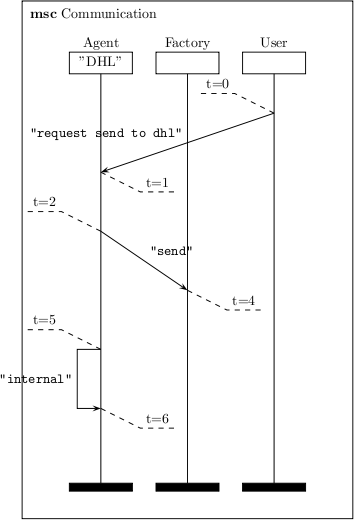
\includegraphics[scale=1]{./images/lars.png}
  \caption{Ejemplo de una comunicación generada con Progtalk}
  \label{fig:lars}
\end{figure}

Para que nuestros BMSCs sean correctos deben cumplir una serie de
requisitos:
\begin{itemize}
\item Los nombres de las instancias deben de ser únicos.
\item Todos los eventos de entrada y salida deben de estar
  relacionados con una instancia ya declarada en el momento del
  evento.
\item Los identificadores de los mensajes deben de ser únicos.
\item Un tiempo de envío no pueden ser nunca mayor que su
  correspondiente tiempo de recepción (ya que no podemos mandar un
  mensaje hacia atrás en el tiempo).
\end{itemize}

%%% Local Variables: 
%%% mode: latex
%%% TeX-master: "progtalk"
%%% TeX-PDF-mode: t
%%% ispell-local-dictionary: "castellano"
%%% End: 
